\documentclass[tikz, border=1mm]{standalone}

\usetikzlibrary{arrows, shapes.gates.logic.US, calc}

\begin{document}
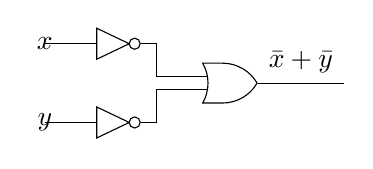
\begin{tikzpicture}
    \node (x) at (0, 1) {$x$};
    \node (y) at (0, 0) {$y$};

    \node[not gate US, draw] at ($(x) + (0.8, 0)$) (notx) {};
    \node[not gate US, draw] at ($(y) + (0.8, 0)$) (noty) {};

    \draw (x) |- (notx.input);
    \draw (y) |- (noty.input);


    \node[or gate US, draw, rotate=0, logic gate inputs=nn] at ($(noty) + (1.5, 0.5)$) (xory) {};

    \draw (notx.output) -- ([xshift=0.2cm]notx.output) |- (xory.input 1);
    \draw (noty.output) -- ([xshift=0.2cm]noty.output) |- (xory.input 2);

    \draw (xory.output) -- node[above]{$\bar x + \bar y$} ($(xory) + (1.5, 0)$);
\end{tikzpicture}
\end{document}
